\chapter{Introduction}

\section{Motivation}



Epidemiology \cite{human_sex}, personal health issues \cite{Madan}, group discovery \cite{5591535}, human mobility \cite{Sun2011929,sevtsuk}, efficient team creation \cite{ECTA, Pentland}, the analysis of academic success \cite{academics}, network theory \cite{networks}, also Fig. \ref{pic:dynamicsf2f}, and psychological research \cite{Rachuri}; all of the above have begun making use of the same notion, one that is difficult to quantify \cite{quant, Wilson}: social connections and social interactions between individuals. And although co-location does not necessarily mean physical social interaction, it is a requirement for it. \cite{Eagle08092009}.

\begin{figure}[h]
	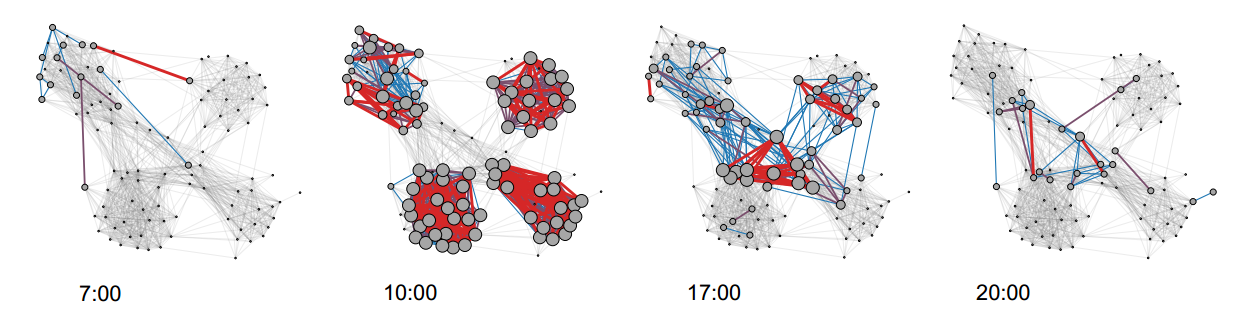
\includegraphics[scale=0.35]{figures/dynamicsf2f.png}
	\caption{Face-to-face interactions over a day for college students. Blue means a low, and red a high frequency of interactions. Image from \protect\cite{Stopczynski}}.
	\label{pic:dynamicsf2f}

\end{figure} 

There are a number of approaches to determining co-location: self-reported data, a more traditional approach, which is prone to cognitive bias, social desirability bias and halo error \cite{Wuchty08092009,gonyea}. A more recent approach involves the use of data provided by modern means of communication, namely mobile phones. This data can come from both the actual phone, in the form of GPS locations or bluetooth readings \cite{Stopczynski}, as well as from the phone company itself in the form of anonymous cell tower records \cite{Onnela01052007, hovel}. This has the advantage of being applicable almost anywhere, because of the high percentage of mobile phone penetration (95.5\% estimated by the International Telecommunication Union in May 2014). 
However, there are approaches that yield better results, but come with financial, environmental or other types of additional cost: RFID tags \cite{catt}, audio-video recordings \cite{audiovideo}, on-body sensors \cite{onbody} and wifi signals \cite{wifi}, just to name a few. 
 
 
\section{Objective}

Given a bluetooth RSSI between two phones, the purpose of this paper is to indicate a method which reliably and accurately determines the existence of pairwise co-location between the people carrying the two phones.

Reliability refers to the fact that multiple tries with the same input, and constant settings ( same machine learning algorithm, same parameters and same training data), will always yield exactly the same result. While accuracy refers to the precision of the algorithm during testing, or how close to the expected result it is. 
 
This inference is achieved by applying and analysing multiple machine learning algorithms on a data set consisting of two main parts:
\begin{itemize}
  \item Data automatically recorded by the SensibleDTU data collector app \cite{Stopczynski}
  \item Ground truth data obtained by the test subjects by interacting with the FriendFinder app
\end{itemize}

For each machine learning algorithm the parameter configuration which yields the best results will be chosen, followed by a comparison between the best configurations for each algorithm.      

\section{Scope and limitations}

The paper analyses the data obtained from three test subjects. Each subject has been given the same phone model, Samsung Galaxy Nexus. The app built for the phones, FriendFinder, has a purely functional purpose. As such, little to no consideration has been given to the style, theme or design of the app. Fig \ref{pic:ff_prtscr} shows the app, and while fir for purpose, it is not very aesthetic.

While considerable testing has been done with regards to the algorithm parameters, the machine learning algorithms list is by no means exhaustive. There are three main algorithms: Naive Bayes, Neural Networks, and Recursive learning, and an explanation on why a fourth, Hidden Markov Model, is unsuitable for this type of data. 

When analysing data, we only look at the bluetooth RSSI value, and data derived directly while measuring it. For example, given that measurements are taken every five minutes, we at some point look at the length of an uninterrupted string of measurements, or at the measurements taken before and after (if possible) a specific measurement. GPS traces, phone records, infrared sensors, or facebook/email information are not taken into consideration.

\section{Thesis Outline}

The thesis begins with this introduction, which gives an overview of the general theme of the project. The objectives, scope and limitations and thesis outline are all self-defining. 

It continues with a section which describes the data acquisition process and the methodology used to obtain the data from the SensibleDTU database. The section also describes the FriendFinder app, as well as its implementation.

Next, the machine learning algorithms are presented. For each algorithm a theoretical overview is given. The implementation details are discussed, followed by the results obtained by applying it to the data. At the end of this chapter, we do a comparative analysis between the algorithms, followed by the last section, the conclusions, where we will give the final results and recommendations.
